%===============================================================================
% ifacconf.tex 2022-02-11 jpuente  
% 2022-11-11 jpuente change length of abstract
% Template for IFAC meeting papers
% Copyright (c) 2022 International Federation of Automatic Control
%===============================================================================
\documentclass{ifacconf}

\usepackage{graphicx}      % include this line if your document contains figures
\usepackage{natbib}        % required for bibliography
%===============================================================================
\begin{document}
\begin{frontmatter}

\title{GEOSPATIAL ANALYSIS FOR THE SELECTION OF ZONES UNDERGROUND STORAGE IN COLOMBIA: SINÚ-SAN JACINTO BASIN CASE\thanksref{footnoteinfo}} 
% Title, preferably not more than 10 words.

\thanks[footnoteinfo]{Sponsor and financial support acknowledgment
goes here. Paper titles should be written in uppercase and lowercase
letters, not all uppercase.}

\author[First]{G.ARIZA, L.} 



\address[First]{Universidad Nacional de Colombia, sede Medellin (e-mail: anggarciaar@unal.edu.co).}


\begin{abstract}                % Abstract of 50--100 words
These instructions give you guidelines for preparing papers for IFAC
technical meetings. Please use this document as a template to prepare
your manuscript. For submission guidelines, follow instructions on
paper submission system as well as the event website.
\end{abstract}

\begin{keyword}
Underground Storage, CO2, Sinu San Jacinto Basin, geospatial analysis
\end{keyword}

\end{frontmatter}
%===============================================================================

\section{Introduction}
In recent years, the imperative to address climate change has necessitated intensified efforts to mitigate greenhouse gas emissions. Carbon capture and storage (CCS) has emerged as a promising strategy, involving the capture and subsurface storage of carbon dioxide (CO2) emissions from industrial processes. However, successful CCS implementation critically hinges upon the identification of optimal zones for underground CO2 storage.

This study focuses on the Sinú-San Jacinto basin and aims to employ geospatial analysis techniques to select a suitable exploration zone for underground CO2 storage. Three key factors will be considered for informed decision-making: proximity to major CO2-emitting cities, the presence of mud volcanoes, and data availability encompassing well data, 2D seismic lines, and 3D seismic data.

Proximity to major CO2-emitting cities within the Sinú-San Jacinto basin constitutes the first factor for evaluation. Selecting a storage zone in close proximity to these urban areas minimizes costs and complexities associated with CO2 transport. Additionally, such proximity presents a more effective solution for reducing carbon footprints in these specific regions\cite{Ajayi2019}.

The presence of mud volcanoes in the Sinú-San Jacinto basin constitutes the second significant factor. These volcanoes, characterized by the emission of natural gases and hot mud, provide indicators of geological activity and subsurface structural variations. Evaluating their presence enhances our understanding of stability and CO2 retention capacities within the selected zone.

Finally, data availability encompassing geospatial data, existing well data, 2D seismic lines, and 3D seismic data in the Sinú-San Jacinto basin represents a crucial factor for analysis. These data sources provide valuable insights into the area's geology, subsurface characteristics, and technical feasibility of underground CO2 storage. Their integration enables comprehensive and precise assessments of potential exploration zones.

By integrating these three factors within the geospatial analysis framework, this study aims to identify an optimal exploration zone in the Sinú-San Jacinto basin that satisfies requirements related to proximity to major CO2-emitting cities, accounts for mud volcano presence, and leverages available data, including well data, 2D seismic lines, and 3D seismic data.

Ultimately, this project aims to provide evidence-based recommendations for stakeholders involved in the implementation of carbon capture and storage technologies within the Sinú-San Jacinto basin. By selecting a suitable zone for underground CO2 storage, this research endeavors to contribute to greenhouse gas emission mitigation efforts and advance towards a more sustainable and climate-resilient future.


\section{Metodology}



\subsection{Data}

In this study, data on CO2 emissions in thousands of metric tons were used, collected by IDEAM. The data considered were taken from the years 1990, 1994, 2000, and 2004 from various sources, including environmental studies conducted by IDEAM, reports submitted to DANE by entities such as the Unidad de Planeación Minero Energética Unit and Ecopetrol, among others, as well as direct estimations and reports provided by some monitoring stations.

The records were obtained using the methodology revised in 1996 by the Intergovernmental Panel on Climate Change (IPCC). This methodology corresponds to an indirect estimation of emissions from different sectors, based on emission factors per unit of consumption or production. The following expression is used to obtain such estimation:

Ecuación

Where:
TE: Total CO2 emissions in the country
A: Activity data of the process in the sector
EF: Emission factor associated with CO2 per unit of activity in the sector

In addition to these data, geological information from the Servicio Geologico de Colombia, geographic information from Google Earth Engine, and the data directory from the Agencia Nacional de Hidrocarburos were also utilized in this study.

\subsection{Models}

\subsubsection{Object-based model}
 In the object perspective, the world is viewed as a collection of spatially located entities. These entities are typically tangible and exist in reality. An object, on the other hand, is a digital representation that captures all or a portion of an entity. Objects are described meticulously, including their boundary lines and other interconnected objects that constitute or are associated with them.
\subsubsection{Field model}
the world is perceived as a dynamic system characterized by properties that exhibit continuous variations across spatial dimensions. This perspective focuses on data that are inherently subject to continuous changes in either two-dimensional or three-dimensional space. In a field, each specific location possesses a value, which can include concepts such as "not here" or zero, and the collective set of values defines the overall field.


\subsection{Data processing}

After conducting several tests in various development environments, it was determined that data processing would be handled using the Google Colab platform, a cloud-based development environment provided by Google. It operates within the framework of Jupyter Notebook and enables users to execute Python code.

During the processing of the data of interest using Python code, multiple Google Colab notebooks were utilized due to interference between certain versions of Numpy and the required libraries for executing different models.

\section{Results}
\subsection{Función Rey..}
Use SI as primary units. Other units may be used as secondary units
(in parentheses). This applies to papers in data storage. For example,
write ``$15\,\mathrm{Gb}/\mathrm{cm}^2$ ($100\,\mathrm{Gb}/\mathrm{in}^2$)''. 
An exception is when
English units are used as identifiers in trade, such as ``3.5 in
disk drive''. Avoid combining SI and other units, such as current in
amperes and magnetic field in oersteds. This often leads to confusion
because equations do not balance dimensionally. If you must use mixed
units, clearly state the units for each quantity in an equation.  The
SI unit for magnetic field strength $\mathbf{H}$ is $\mathrm{A}/\mathrm{m}$. However, if you wish to
use units of $\mathrm{T}$, either refer to magnetic flux density $\mathbf{B}$ or
magnetic field strength symbolized as $\mu_0\,\mathbf{H}$. Use the center dot to
separate compound units, e.g., ``$\mathrm{A} \cdot \mathrm{m}^2$''.

\section{Discussion}

\subsection{Figures and Tables}

Figure axis labels are often a source of confusion. Use words rather
than symbols. As an example, write the quantity ``Magnetization'', or
``Magnetization M'', not just ``M''. Put units in parentheses. Do not
label axes only with units.  For example, write ``Magnetization
($\mathrm{A}/\mathrm{m}$)'' or ``Magnetization ($\mathrm{A} \mathrm{m}^{-1}$)'', not just
 ``$\mathrm{A}/\mathrm{m}$''. Do not
label axes with a ratio of quantities and units. For example, write
``Temperature ($\mathrm{K}$)'', not ``$\mbox{Temperature}/\mathrm{K}$''.

Multipliers can be especially confusing. Write ``Magnetization
($\mathrm{kA}/\mathrm{m}$)'' or ``Magnetization ($10^3 \mathrm{A}/\mathrm{m}$)''. Do not write
``Magnetization $(\mathrm{A}/\mathrm{m}) \times 1000$'' because the reader would not know
whether the axis label means $16000\,\mathrm{A}/\mathrm{m}$ or $0.016\,\mathrm{A}/\mathrm{m}$.

\begin{figure}
	\centering
	\includegraphics[width=1\linewidth]{"img/Kernel Desnsity de Volcanes de lodo"}
	\caption[KDvolcanes]{Mapa de analisis de Kernel}
	\label{fig:kernel-desnsity-de-volcanes-de-lodo}
\end{figure}
\begin{figure}
	\centering
	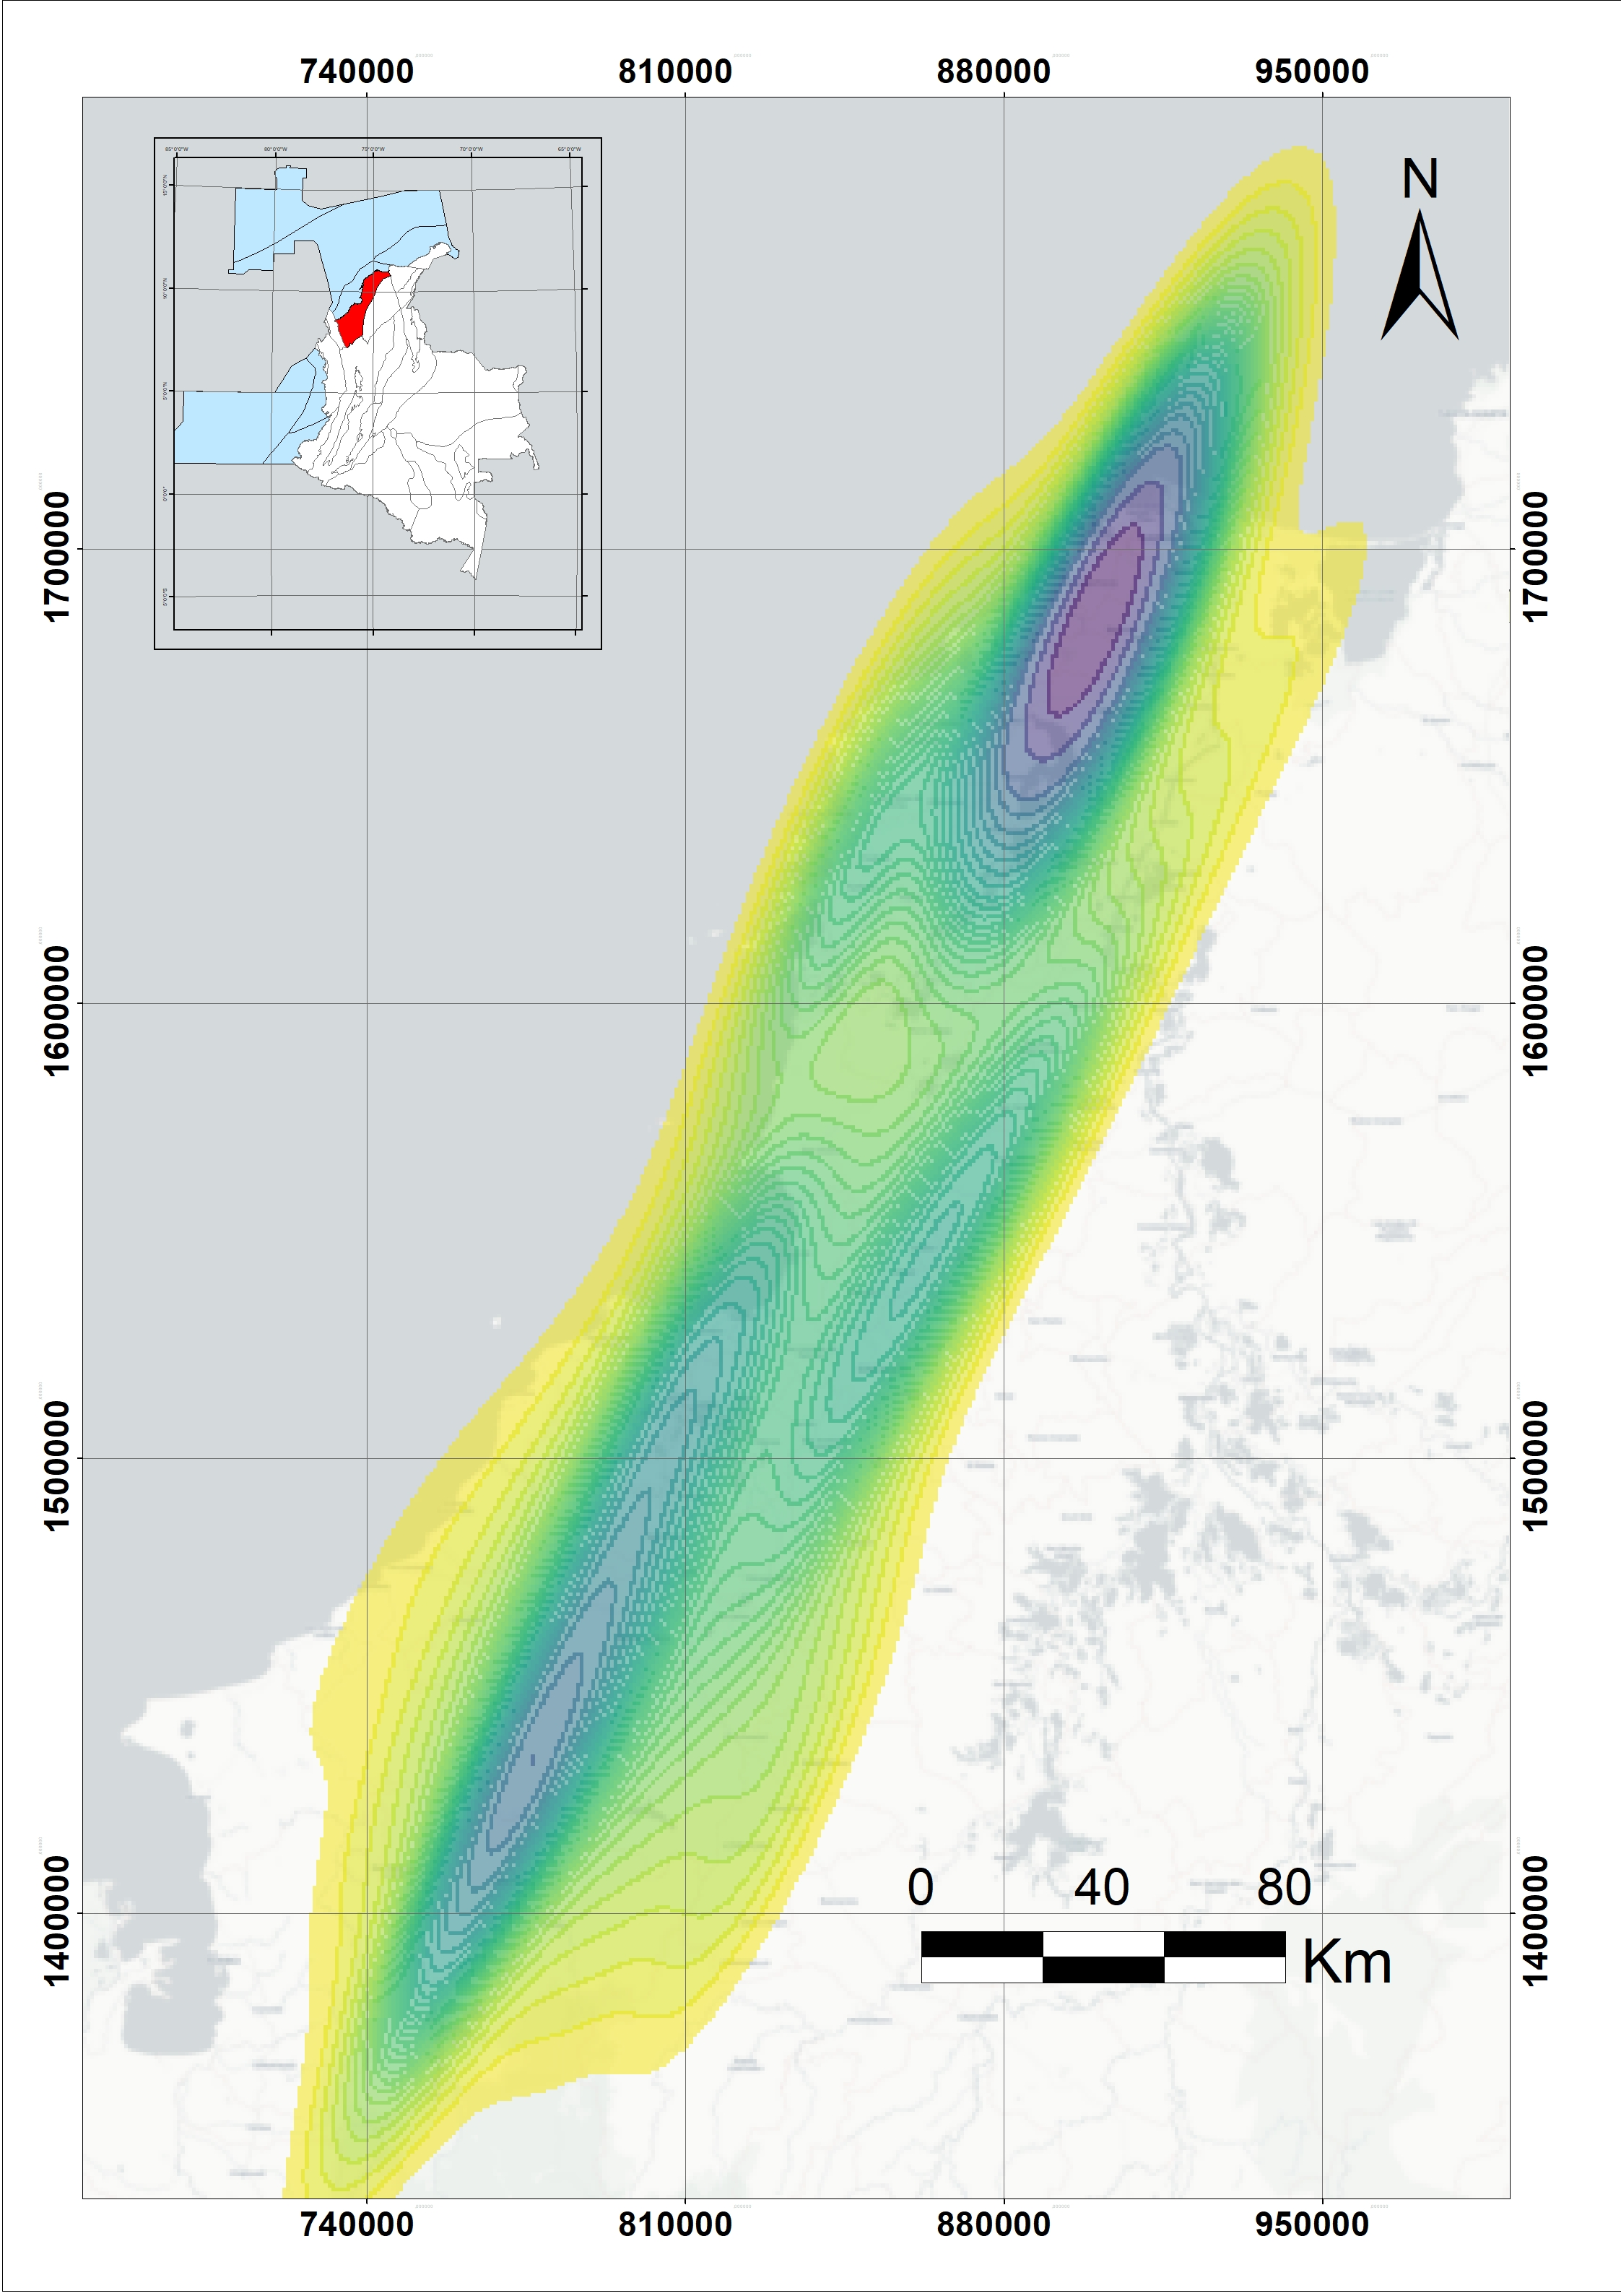
\includegraphics[width=0.7\linewidth]{img/Kernel_Desnsity_Pozos}
	\caption[KDpozos]{}
	\label{fig:kerneldesnsitypozos}
\end{figure}
\begin{figure}
	\centering
	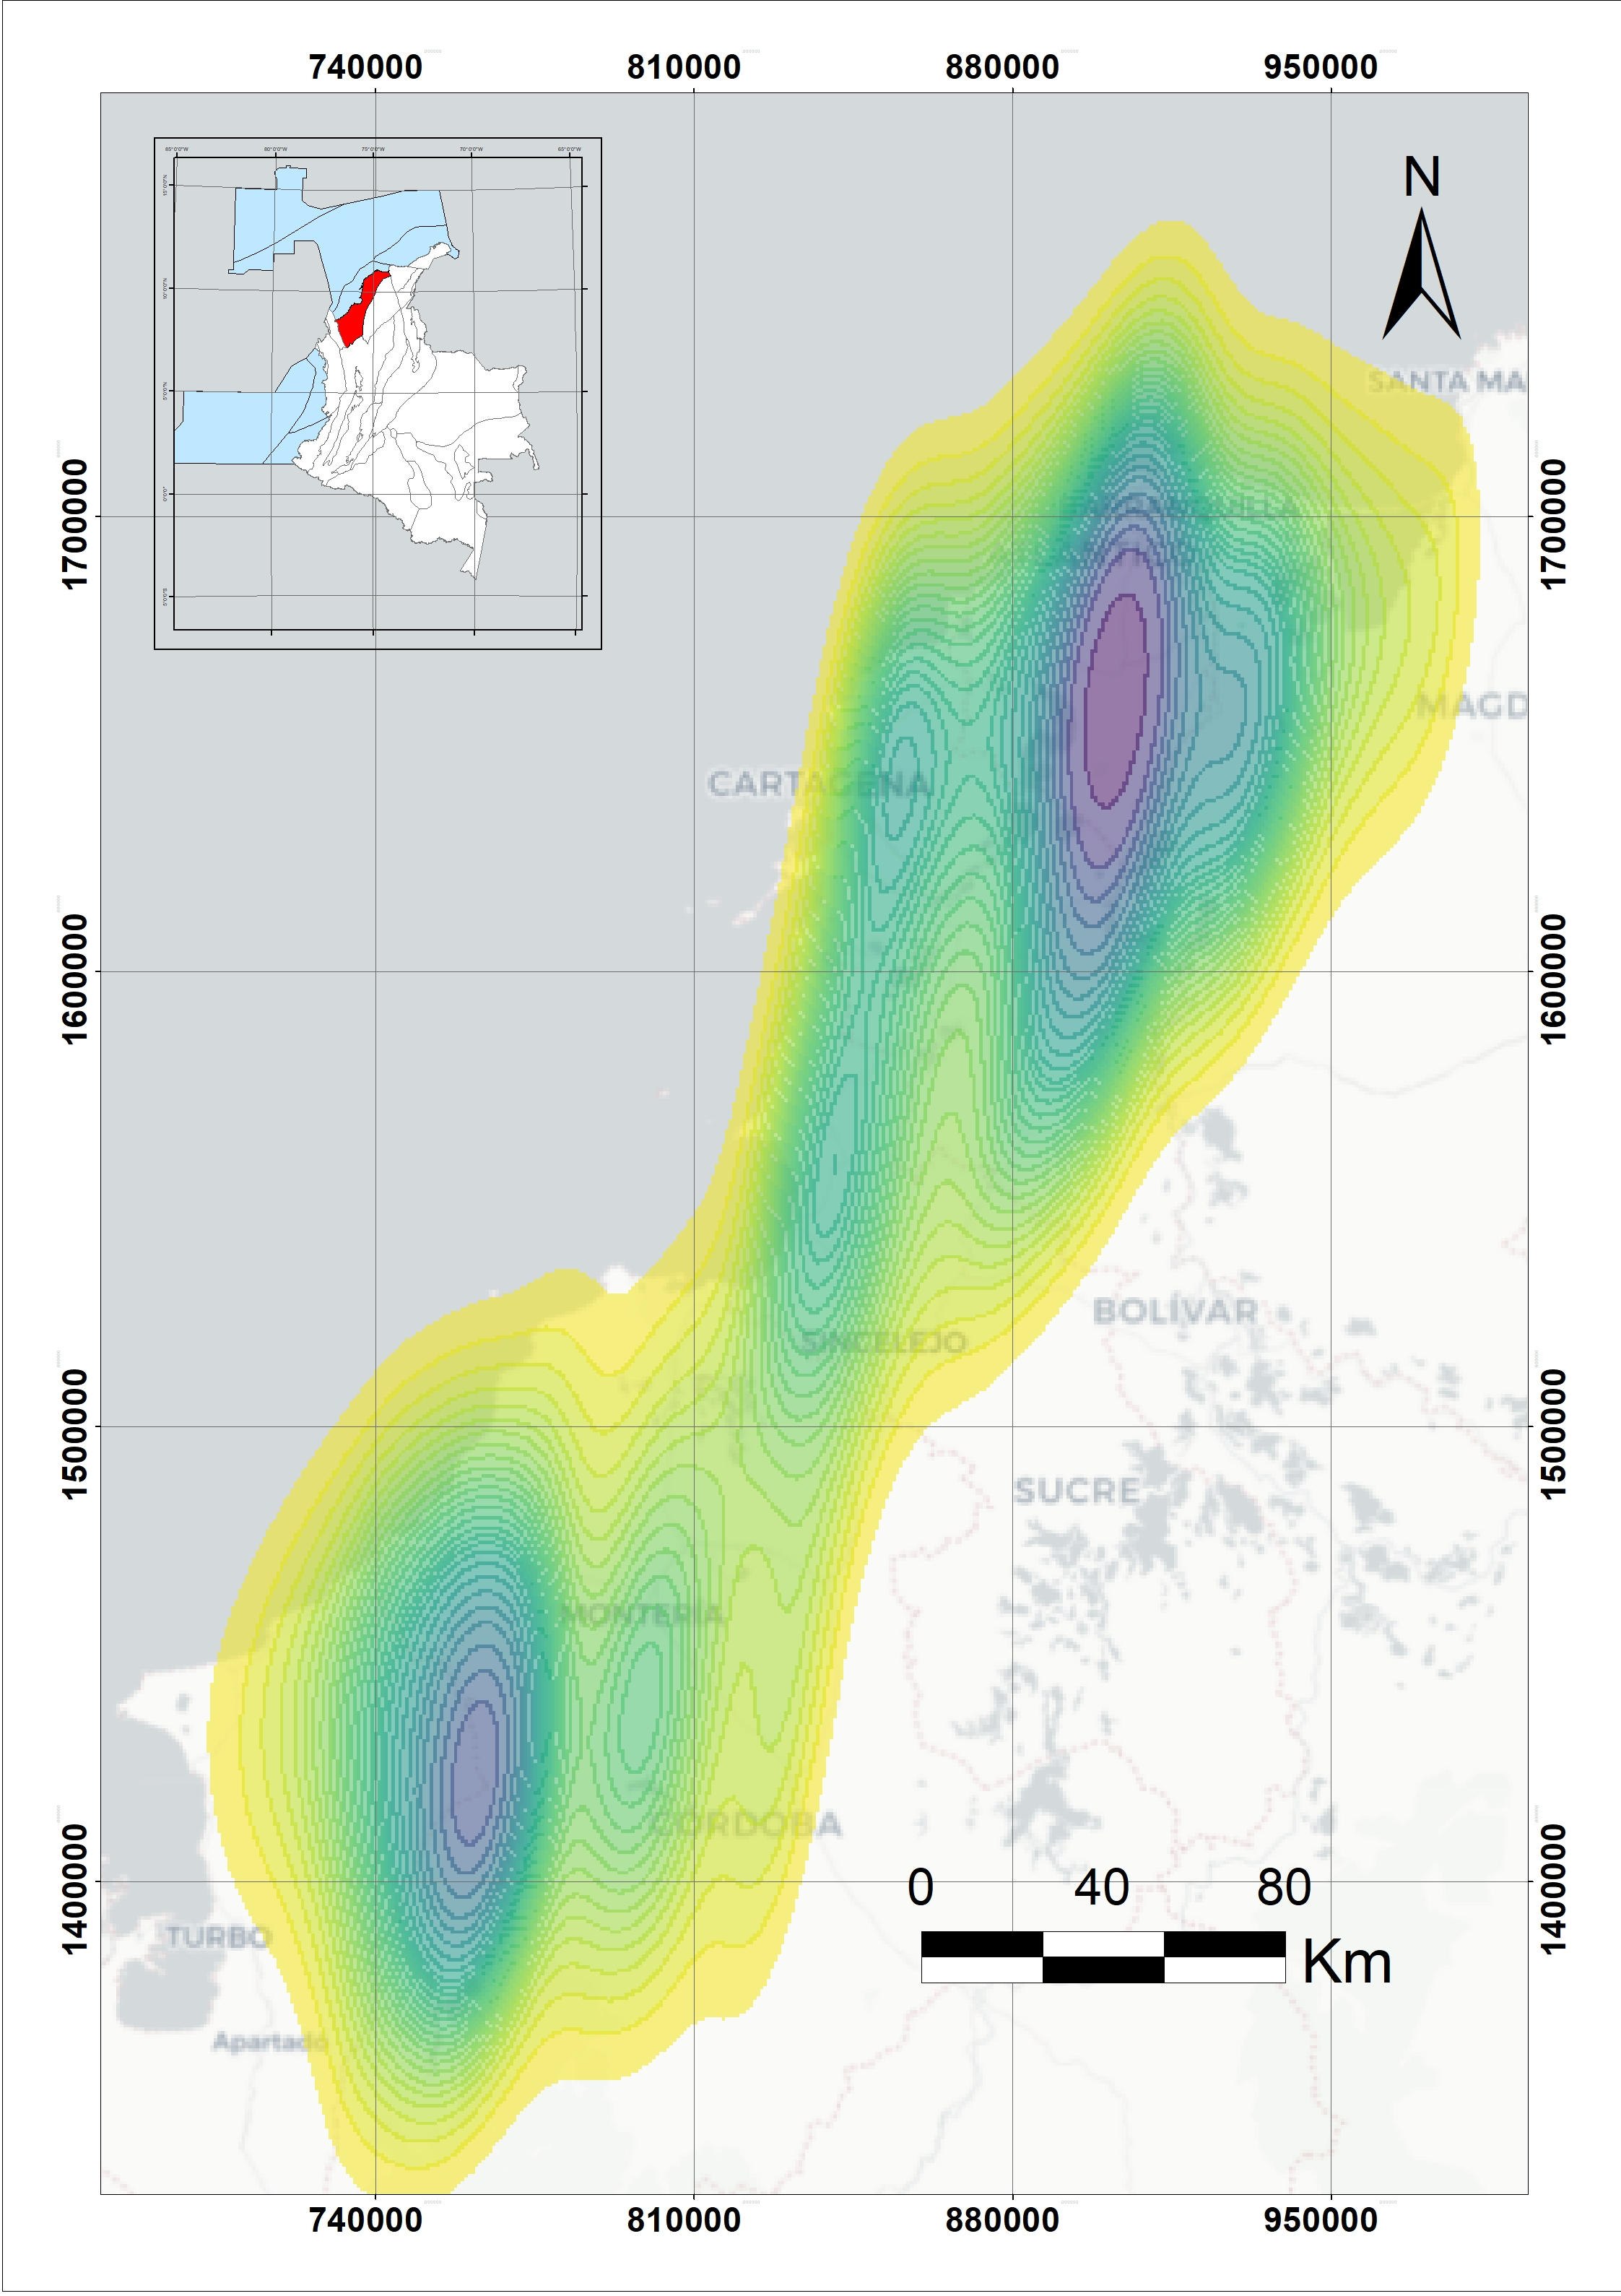
\includegraphics[width=0.7\linewidth]{img/Lineas2D_kde}
	\caption[KDlineas2d]{}
	\label{fig:lineas2dkde}
\end{figure}
\begin{figure}
	\centering
	\includegraphics[width=0.7\linewidth]{"img/Mapa cubo sismico"}
	\caption[mapa3dsismica]{}
	\label{fig:mapa-cubo-sismico}
\end{figure}
\begin{figure}
	\centering
	\includegraphics[width=0.7\linewidth]{"img/mapa de emiciones"}
	\caption[mapaemisiones]{}
	\label{fig:mapa-de-emiciones}
\end{figure}
\begin{figure}
	\centering
	\includegraphics[width=0.7\linewidth]{"img/Mapa de Pozos"}
	\caption[mapapozos]{}
	\label{fig:mapa-de-pozos}
\end{figure}
\begin{figure}
	\centering
	\includegraphics[width=0.7\linewidth]{"img/Mapa de sismica 2D"}
	\caption[mapasismica2d]{}
	\label{fig:mapa-de-sismica-2d}
\end{figure}
\begin{figure}
	\centering
	\includegraphics[width=0.7\linewidth]{"img/Sin título"}
	\caption[centroidesemisiones]{}
	\label{fig:sin-titulo}
\end{figure}
\begin{figure}
	\centering
	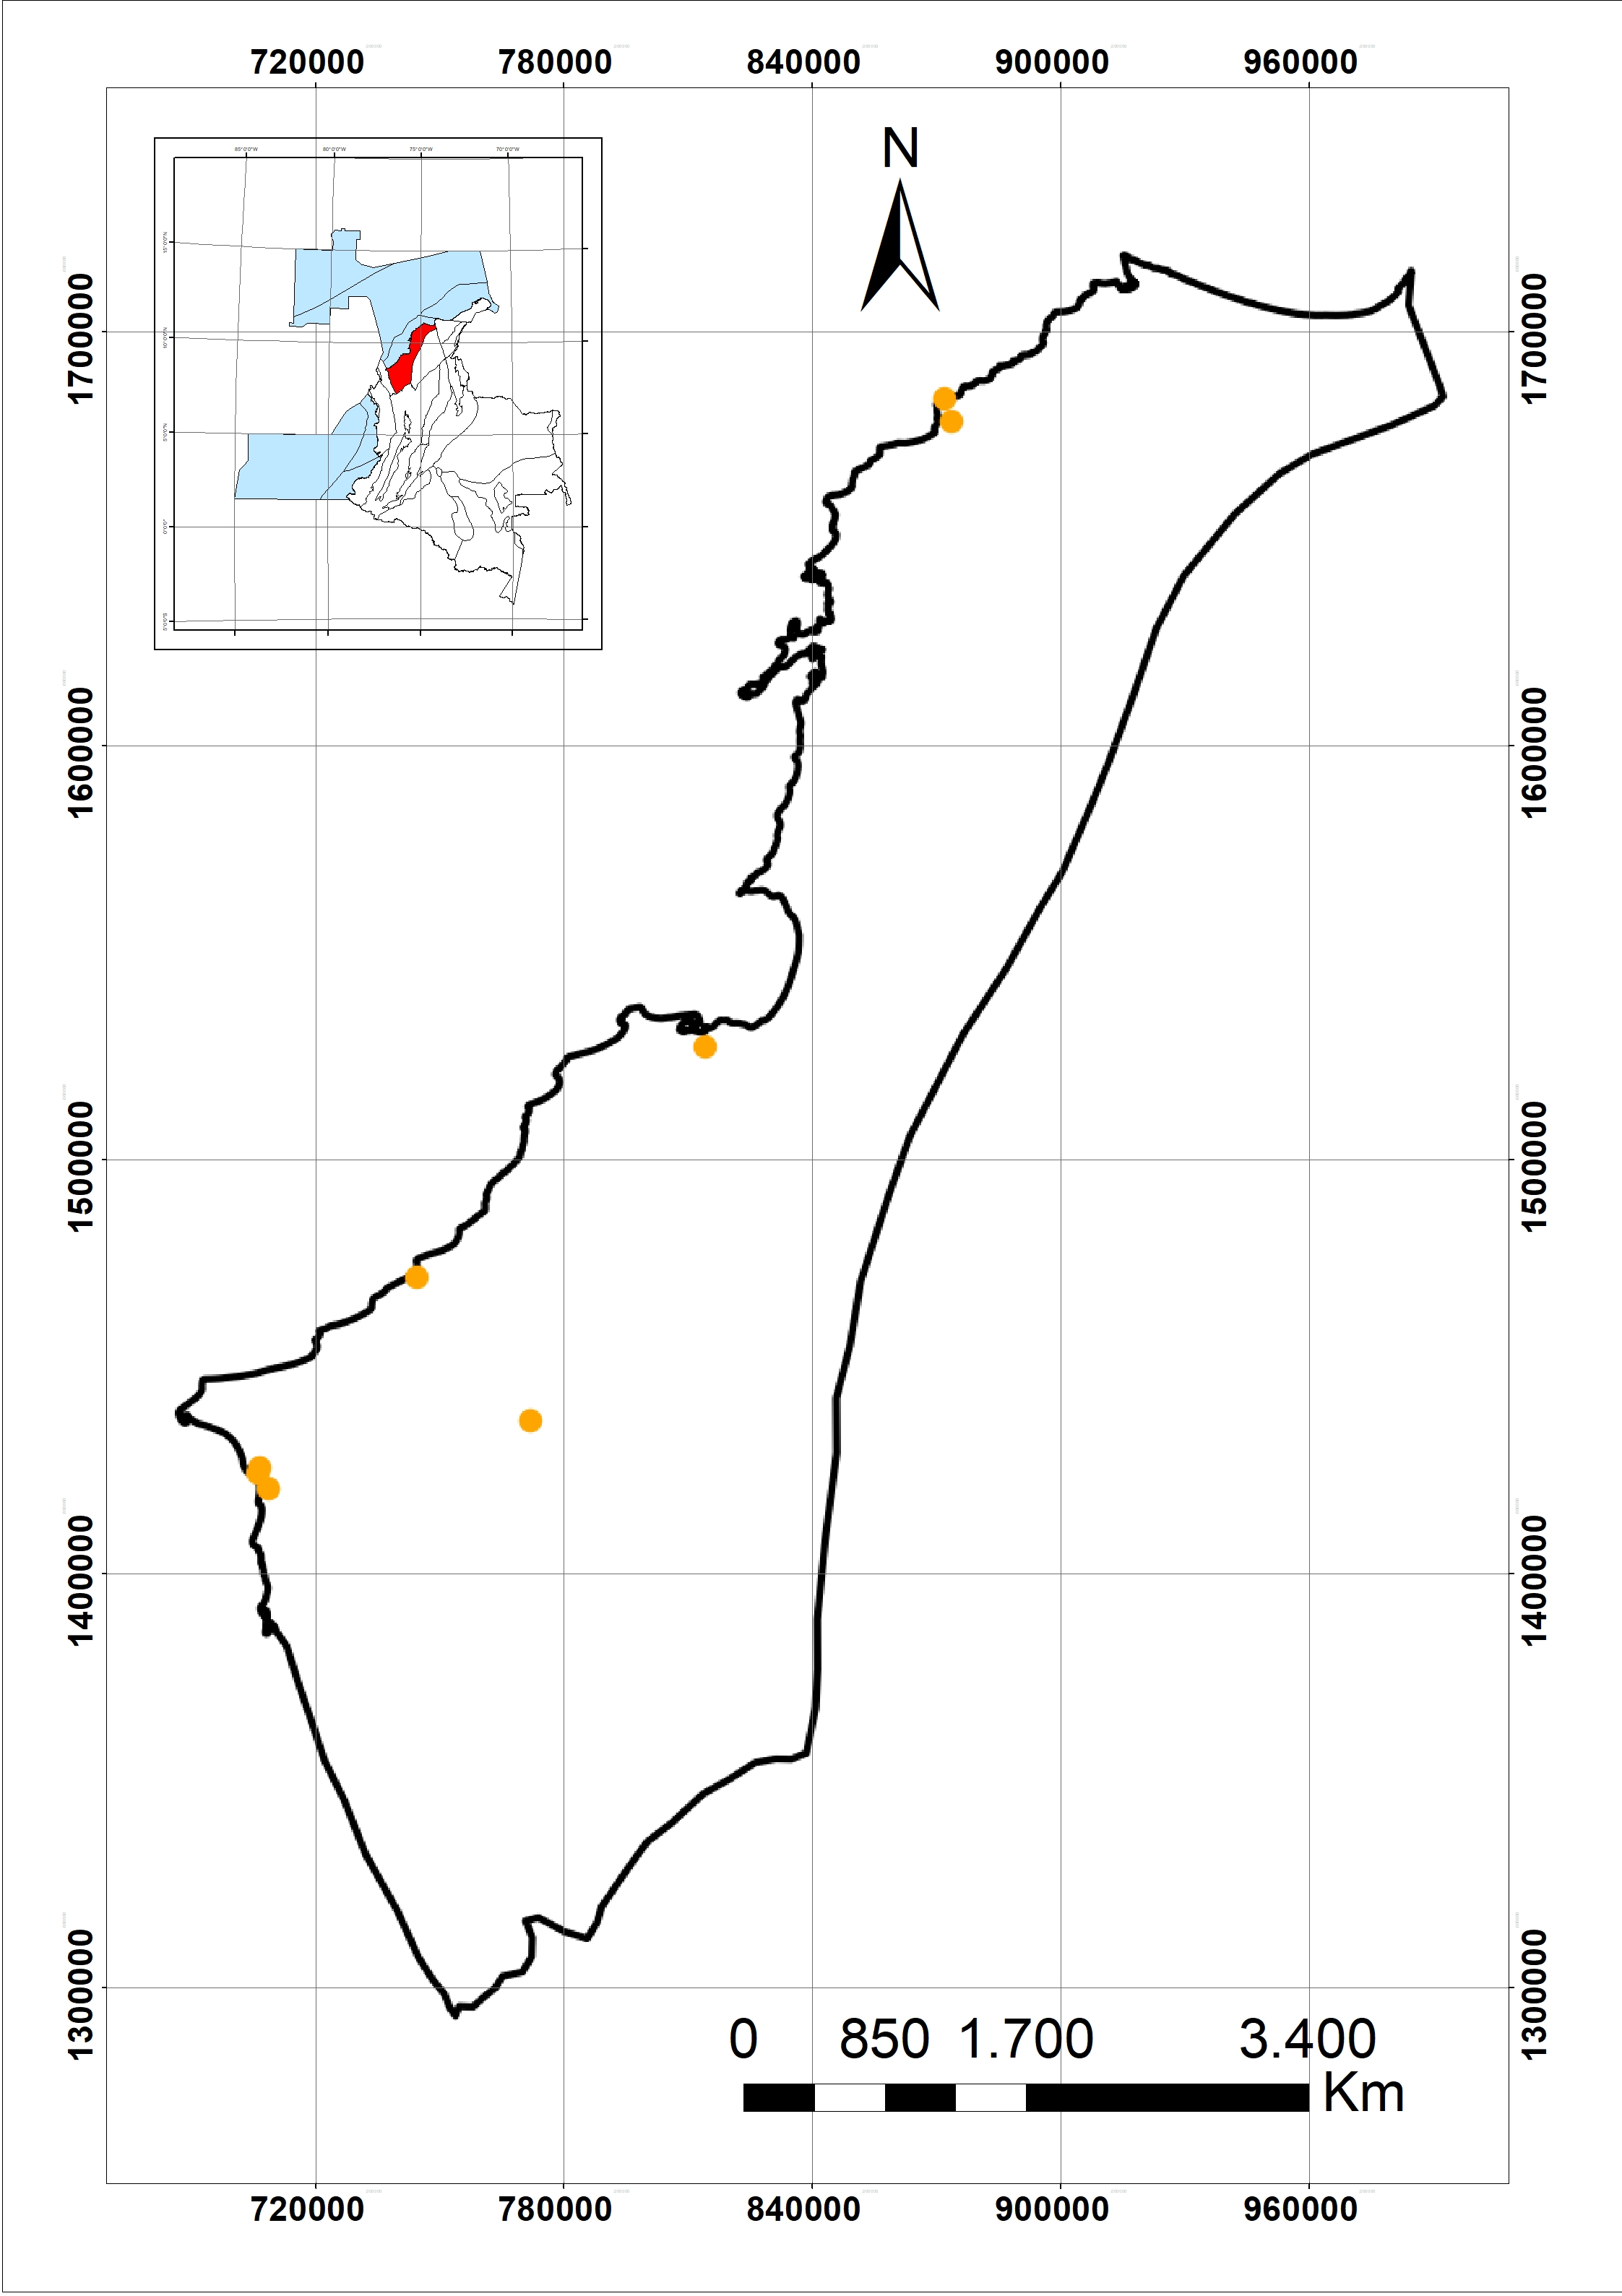
\includegraphics[width=0.7\linewidth]{img/Volcanes}
	\caption[volcanes]{}
	\label{fig:volcanes}
\end{figure}


\subsection{References}

Use Harvard style references (see at the end of this document). With
\LaTeX, you can process an external bibliography database 
using \texttt{bibtex},\footnote{In this case you will also need the \texttt{ifacconf.bst}
file, which is part of the \texttt{ifaconf} package.}
or insert it directly into the reference section. Footnotes should be avoided as
far as possible.  Please note that the references at the end of this
document are in the preferred referencing style. Papers that have not
been published should be cited as ``unpublished''.  Capitalize only the
first word in a paper title, except for proper nouns and element
symbols.

\subsection{Abbreviations and Acronyms}

Define abbreviations and acronyms the first time they are used in the
text, even after they have already been defined in the
abstract. Abbreviations such as IFAC, SI, ac, and dc do not have to be
defined. Abbreviations that incorporate periods should not have
spaces: write ``C.N.R.S.'', not ``C. N. R. S.'' Do not use abbreviations
in the title unless they are unavoidable (for example, ``IFAC'' in the
title of this article).

\subsection{Equations}

Number equations consecutively with equation numbers in parentheses
flush with the right margin, as in (\ref{eq:sample}).  To make your equations more
compact, you may use the solidus ($/$), the $\exp$ function, or
appropriate exponents. Use parentheses to avoid ambiguities in
denominators. Punctuate equations when they are part of a sentence, as
in

\begin{equation} \label{eq:sample2}
\begin{array}{ll}
\int_0^{r_2} & F (r, \varphi ) dr d\varphi = [\sigma r_2 / (2 \mu_0 )] \\
& \cdot \int_0^{\inf} exp(-\lambda |z_j - z_i |) \lambda^{-1} J_1 (\lambda  r_2 ) J_0 (\lambda r_i ) d\lambda 
\end{array}
\end{equation}

Be sure that the symbols in your equation have been defined before the
equation appears or immediately following. Italicize symbols ($T$
might refer to temperature, but T is the unit tesla). Refer to
``(\ref{eq:sample})'', not ``Eq. (\ref{eq:sample})'' or ``equation
(\ref{eq:sample})'', except at the beginning of a sentence: ``Equation
(\ref{eq:sample}) is \ldots''.

\subsection{Other Recommendations}

Use one space after periods and colons. Hyphenate complex modifiers:
``zero-field-cooled magnetization''. Avoid dangling participles, such
as, ``Using (1), the potential was calculated'' (it is not clear who or
what used (1)). Write instead: ``The potential was calculated by using
(1)'', or ``Using (1), we calculated the potential''.

A parenthetical statement at the end of a sentence is punctuated
outside of the closing parenthesis (like this). (A parenthetical
sentence is punctuated within the parentheses.) Avoid contractions;
for example, write ``do not'' instead of ``don' t''. The serial comma
is preferred: ``A, B, and C'' instead of ``A, B and C''.


\section{Conclusion}

A conclusion section is not required. Although a conclusion may review
the main points of the paper, do not replicate the abstract as the
conclusion. A conclusion might elaborate on the importance of the work
or suggest applications and extensions.

\begin{ack}
Place acknowledgments here.
\end{ack}

\bibliography{ifacconf}             % bib file to produce the bibliography
                                                     % with bibtex (preferred)
                                                   
%\begin{thebibliography}{xx}  % you can also add the bibliography by hand

%\bibitem[Able(1956)]{Abl:56}
%B.C. Able.
%\newblock Nucleic acid content of microscope.
%\newblock \emph{Nature}, 135:\penalty0 7--9, 1956.

%\bibitem[Able et~al.(1954)Able, Tagg, and Rush]{AbTaRu:54}
%B.C. Able, R.A. Tagg, and M.~Rush.
%\newblock Enzyme-catalyzed cellular transanimations.
%\newblock In A.F. Round, editor, \emph{Advances in Enzymology}, volume~2, pages
%  125--247. Academic Press, New York, 3rd edition, 1954.

%\bibitem[Keohane(1958)]{Keo:58}
%R.~Keohane.
%\newblock \emph{Power and Interdependence: World Politics in Transitions}.
%\newblock Little, Brown \& Co., Boston, 1958.

%\bibitem[Powers(1985)]{Pow:85}
%T.~Powers.
%\newblock Is there a way out?
%\newblock \emph{Harpers}, pages 35--47, June 1985.

%\bibitem[Soukhanov(1992)]{Heritage:92}
%A.~H. Soukhanov, editor.
%\newblock \emph{{The American Heritage. Dictionary of the American Language}}.
%\newblock Houghton Mifflin Company, 1992.

%\end{thebibliography}

\appendix
\section{A summary of Latin grammar}    % Each appendix must have a short title.
\section{Some Latin vocabulary}              % Sections and subsections are supported  
                                                                         % in the appendices.
\end{document}
